\section{Method}
\label{sec:method}

\subsection{High-level Architecture}
In figure \ref{fig:highLevelArchitecture} the main components of the architecture used can be seen.
For this project the \textit{input} data consist of a sequence of images, where we use the dataset presented in section \ref{sec:dataset} where the region-of-interest is extracted.
The \textit{visual model} is used to extracting features from the input data and the \textit{temporal model} is used to correlate these features in time.
The \textit{output} is generated by classifying the input sequence to a particular class.

\begin{figure}
    \centering
    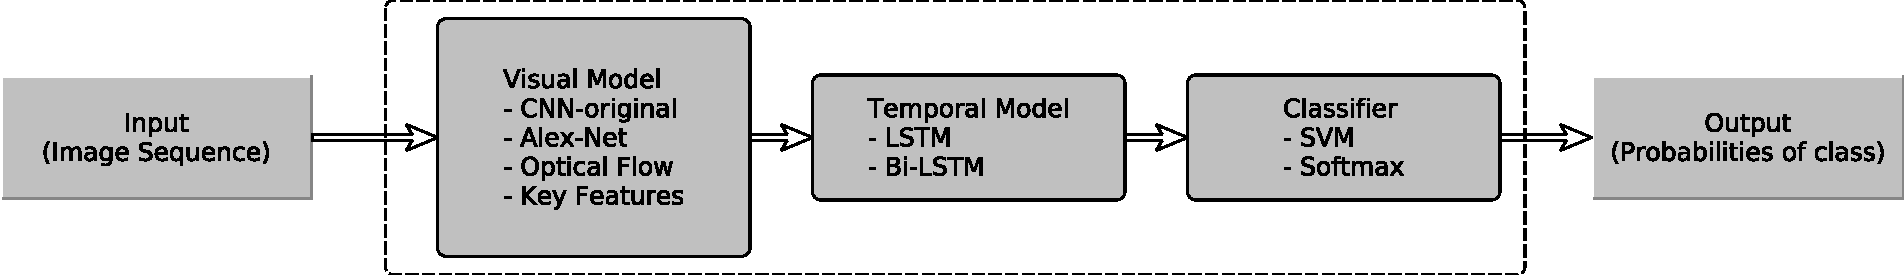
\includegraphics[width=\columnwidth]{fig/highLevelArchitecture.jpg}
    \caption{High-level architecture used}
    \label{fig:highLevelArchitecture}
\end{figure}

\subsection{Proposed Architecture}
We propose to use serial different model for both the visual model en the temporal model.
We will here implement and evaluate each of these models to see how they perform and compare this to the current state-of-the-art architecture.
We will here use the visual and temporal models listed in table \ref{tab:visualTemporalModel}.

\begin{table}
\centering
\begin{tabular}{l|l}
Visual Model & Temporal Model\\
\hline
CNN-original & LSTM\\
Alex-net & B-LSTM\\
Optical Flow & \\
Key Features &
\end{tabular}
\caption{Table with the different Visual and Temporal models used}
\label{tab:visualTemporalModel}
\end{table}

From these visual and temporal models a total of 10 different architectures can be obtained by combining a single visual model with a single temporal model.
Beside these 10 different architecture further can be obtained by combining multiple visual models with a single temporal model.
I our approach we will first obtain results from the 10 basic models and then 


Temporal Model
LSTM
B-LSTM


Alex-net + LSTM
CNN-original + Bidirectional LSTM
Optical flow + LSTM
Key features + LSTM

